\begin{tabular}{cc}
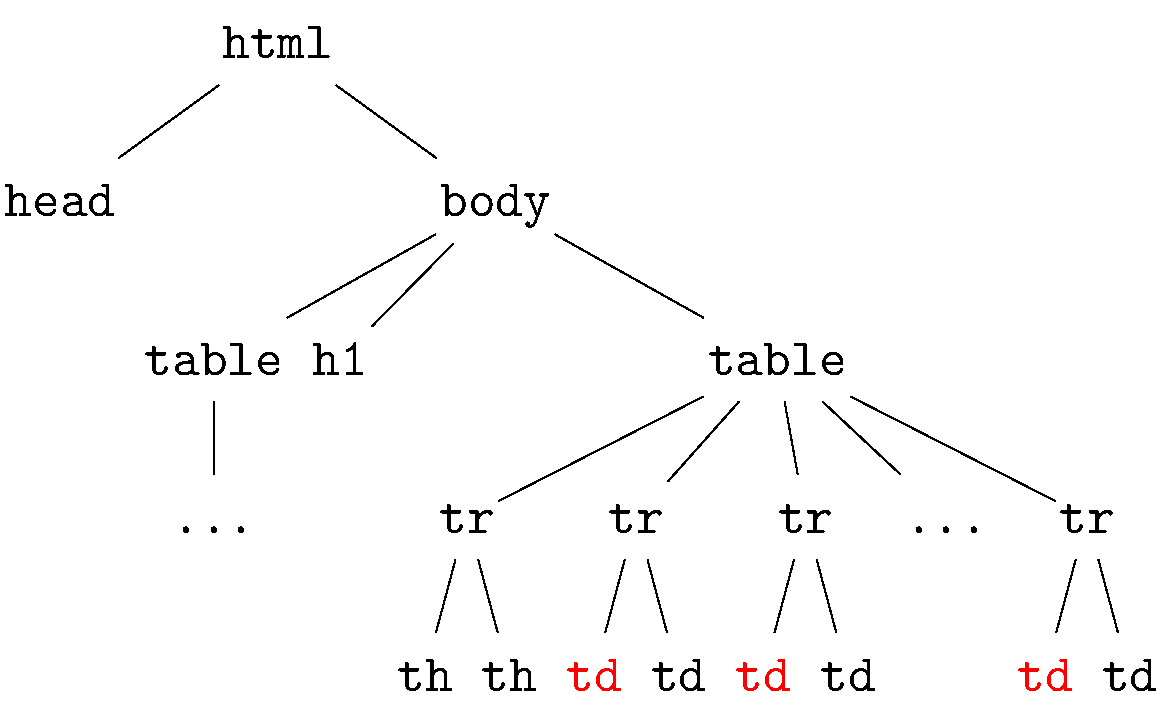
\includegraphics[scale=0.35]{sfig/openweb.slides/extractionFeatureStructural} &
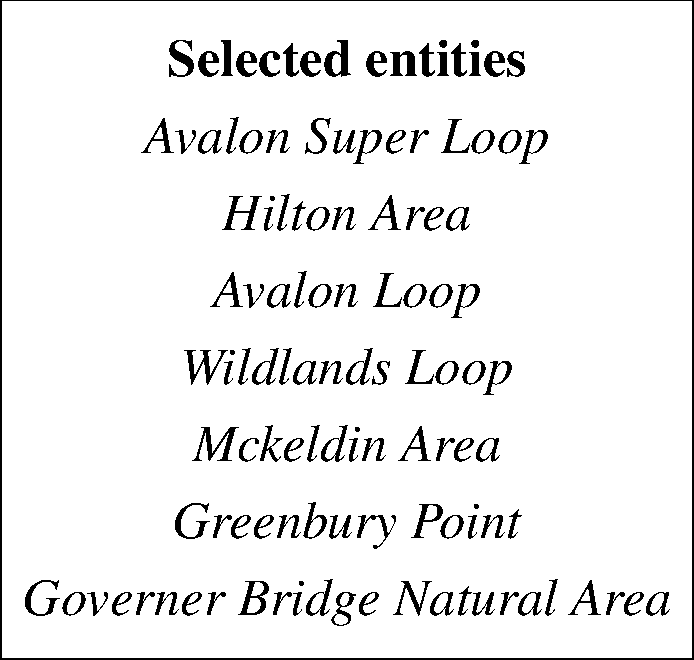
\includegraphics[scale=0.35]{sfig/openweb.slides/extractionFeatureDenotation} \\
\begin{tabular}[t]{ll} \toprule
\textbf{Structural feature} & \textbf{Value} \\ \midrule 
Features on selected nodes: \\
\quad\textsc{Tag-Majority} = \texttt{td} & 1\\
\quad\textsc{Index-Entropy} & 0.0 \\
Features on parent nodes: \\
\quad\textsc{ChildrenCount-Majority} = 2 & 1 \\
\quad\textsc{Parent-Single} & 1\\
\quad\textsc{Index-Entropy} & 1.0 \\
\quad\textsc{HeadHole} {\small (The first node is skipped)} & 1\\
Features on grandparent nodes: \\
\quad\textsc{PageCoverage} & 0.6 \\
\ldots & \ldots \\
\bottomrule
\end{tabular} &
\begin{tabular}[t]{ll} \toprule
\textbf{Denotation feature} & \textbf{Value} \\ \midrule 
\textsc{WordsCount-Mean} & 2.42 \\
\textsc{PhraseShape-Majority} = \texttt{Aa Aa} & 1 \\
\textsc{PhraseShape-MajorityRatio} & 0.71 \\
\textsc{WordShape-Majority} = \texttt{Aa} & 1 \\
\textsc{PhrasePOS-Majority} = NNP NN & 1\\
\textsc{LastWord-Entropy} & 0.74 \\ 
\textsc{WordPOS} = NN {\small (normalized count)} & 0.53 \\
\ldots & \ldots \\
\bottomrule
\end{tabular}
\end{tabular}
